\section{Diagram klas}
\subsection{Rysunek (diagram)}
\begin{figure}[!htb]
    \centering
    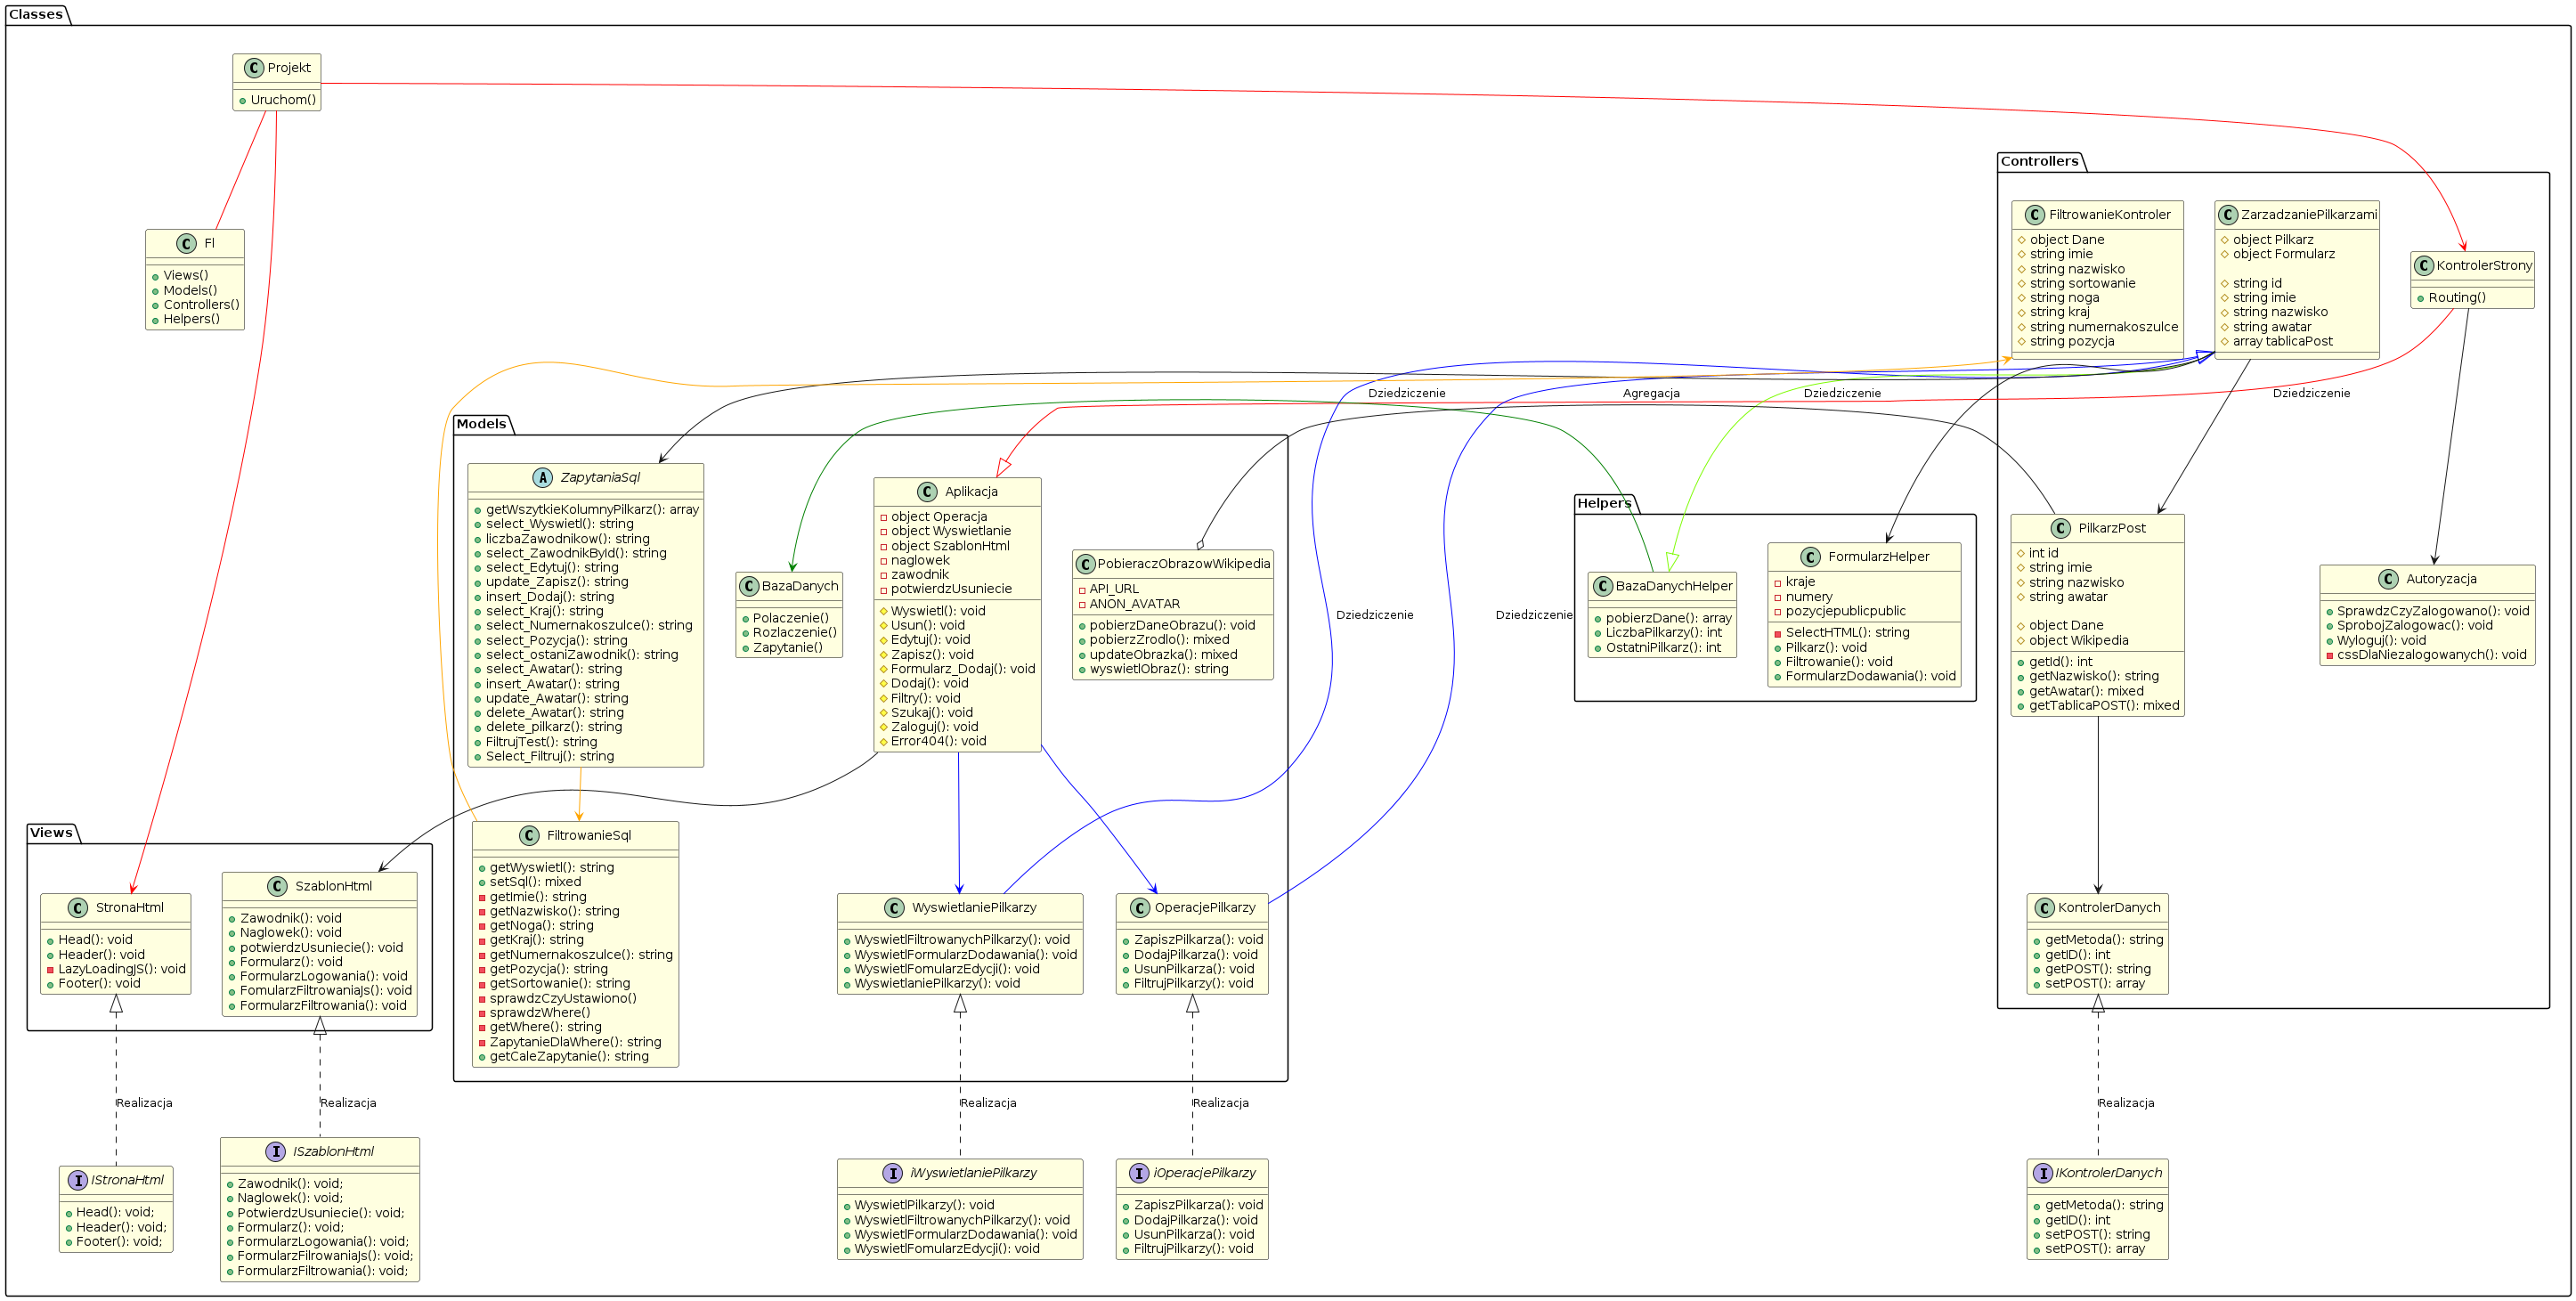
\includegraphics[width=1.0\textwidth]{diagramy/klas.png}
    \caption{Diagram klas}                
\end{figure}

\subsection{Opis przeznaczenia klas}
    Klasy są segregowane według modelu \textbf{MVC} i pomocniczych klas opisanych jako \textbf{Helpers}

\subsection{Models}
    \subsubsection{Aplikacja}
    \subsubsection{BazaDanych}
    \subsubsection{ZapytaniaSql}
    \subsubsection{FiltrowanieSql}
    \subsubsection{OperacjePilkarzy}
    \subsubsection{WyswietlaniePilkarzy}
    \subsubsection{PobieraczObrazowWikipedia}
        Klasa za pomocą otwartego API Wikipedia, pobiera adres URL do głównego zdjęcia piłkarza z artykułu na Wikipedii. Zdjęcie jest pobierane podczas dodawania nowego piłkarza bądź jego edycji i zapisywana w bazie danych w taleli "awatar" w postaci linku.
    \subsection{Controllers}
        \subsubsection{Autoryzacja}
        \subsubsection{FiltrowanieKontroler}
        \subsubsection{KontrolerDanych}
            Ta klasa służy do odbierania danych od użytkownika z poziumu aplikacji, używając metod GET (parametry z linku ) oraz POST (niejawnych, przesyłanych z formularzy.)
        \subsubsection{PilkarzPost}
        \subsubsection{Autoryzacja}
        \subsubsection{ZarzadzaniePilkarzami}

    \subsection{Views}
        \subsubsection{StronaHtml}
        Zawiera szkielet strony HTML, taki jak sekcja <head> <body> <footer> czy <header>. Dzięki temu rozwiązaniu można ustawić Podstawowe dane takie jak tytuł strony, autorów, w kiklu miejscach na stronie, wczytywana z pliku konfiguracyjnego \textbf{KonfiguracjaApp.php}
        \subsubsection{SzablonHtml}

    \subsection{Helpers}
        \subsubsection{BazaDanychHelper}
        \subsubsection{FormularzHelper}
        
    \subsection{Projekt}
        \lstinputlisting{./src/code_snippets/Projekt.php}  

    \subsection{FileLoader}